% Generated by tools/paper/render.py from main_text.py; edit the source there, not this file.
\documentclass[numsec,webpdf,modern,large]{oup-authoring-template}
\usepackage{booktabs}
\usetikzlibrary{plotmarks}
\tikzset{box/.style={draw, rounded corners=2pt, align=center, font=\footnotesize, inner sep=3pt}, inbox/.style={box, fill=gray!10}, outbox/.style={box, fill=gray!10, very thick}, arr/.style={-latex, thick}}
\begin{document}
\journaltitle{Bioinformatics}
\DOI{DOI added during production}
\copyrightyear{2026}
\pubyear{2026}
\access{Published: Date added during production}
\appnotes{Original Paper}
\firstpage{1}
\title[pgphase]{pgphase: phasing long reads at a pangenome's known alleles and the sample's own heterozygous variants}
\author[1,$\ast$]{Konstantinos Kyriakidis}
\address[1]{\orgname{UC Santa Cruz Genomics Institute}, \orgaddress{\state{Santa Cruz, CA}, \country{USA}}}
\corresp[$\ast$]{Corresponding author. \href{mailto:kkyriaki@ucsc.edu}{kkyriaki@ucsc.edu}}
\received{Date}{0}{Year}
\revised{Date}{0}{Year}
\accepted{Date}{0}{Year}
% Generated by tools/paper/render.py from main_text.py; edit the source there, not this file.
\abstract{\textbf{Motivation:} Read-based phasers assign the heterozygous variants of a diploid genome, and the long reads that carry them, to the two parental haplotypes. They phase the variants a caller found on a linear reference: where the caller misses the heterozygous variants of a region its reads are left unphased, and where it calls the differences between copies of a collapsed duplication as heterozygous, they are phased against one another and join blocks in the wrong orientation. Applications that use the reads themselves, such as haplotype-resolved assembly and allele-specific analyses, depend on how many reads are phased, and phased correctly.\\
\textbf{Results:} We present pgphase, which phases reads at the known alleles of a pangenome graph, observed through the reads' own graph alignments without calling them, together with the heterozygous variants the sample carries outside the graph, found in its linear alignments. One expectation-maximization over both learns each site's error rate, and blocks are joined only where several reads verify the join. On HG002 PacBio HiFi reads aligned to the Human Pangenome Reference Consortium graph, with the parent of origin of every read as truth, on eight chromosomes of which three were held out from development, pgphase phased 99.08\% of 2{,}623,162 phaseable reads correctly, against 94.41\% for the best of HiPhase, LongPhase, WhatsHap and longcallD. It left 6.1 times fewer reads misphased or unphased than HiPhase, made 58 switch errors against 105 for the best of them, and phased more truth heterozygous variants than any phaser given DeepVariant's calls.\\
\textbf{Availability and implementation:} pgphase is free software under the MIT license, available at \url{https://github.com/kokyriakidis/pgphase}.}

\keywords{phasing, haplotagging, long reads, pangenome graph, graph alignment, expectation maximization}
\maketitle
% Generated by tools/paper/render.py from main_text.py; edit the source there, not this file.
\section{Introduction}

A long read spans several heterozygous variants, so the reads of a diploid sample and its heterozygous variants can be phased together: each read is assigned to the parental haplotype it was sequenced from, and each variant allele to the haplotype whose reads carry it \citep{Patterson2015,Edge2017}. Phased variants give haplotypes; phased reads, tagged with their haplotype, are themselves the input of haplotype-resolved analyses, from allele-specific methylation and expression to the local assembly and structural variant calling of each haplotype. Accurate long reads such as PacBio HiFi \citep{Wenger2019} make this possible on a single sample.

Read-based phasers differ in how they solve the problem. WhatsHap minimises the number of read alleles that must be corrected for the reads to split into two haplotypes \citep{Patterson2015,Martin2016}, HapCUT2 maximises a likelihood by iterated cuts \citep{Edge2017}, LongPhase finds the two heaviest disjoint paths through a graph of variants linked by reads, and phases structural variants with them \citep{Lin2022}, and HiPhase searches with A* and phases small, structural and tandem repeat variants jointly \citep{Holt2024}. Each phases a set of variants a caller found on a linear reference, typically DeepVariant \citep{Poplin2018,Shafin2021}; longcallD calls and phases variants together, resolving noisy regions with local multiple sequence alignment \citep{Gao2026}.

Phasing from a linear reference has two blind spots that matter for the reads more than for the variants. Where the caller finds no heterozygous variant, in tandem repeats and other regions where read alignments disagree, the reads have nothing to be phased by and are left unphased. Where a region is duplicated in the sample but not in the reference, the reads of both copies align to one place, and the copies' differences look like heterozygous variants: they co-segregate as perfectly as real ones, and the reads they label, and the blocks they join, can be phased in the wrong orientation by the thousand. Phasers are usually compared by their phased variants, through switch errors and block lengths \citep{Lin2022,Holt2024}, which count neither the reads left unphased nor a block of reads joined wrongly by a few variants.

A pangenome graph describes the known alleles of many genomes at once \citep{Liao2023,Hickey2024}, and graph aligners place reads on it \citep{Garrison2018,Siren2021}. Where a read crosses a site of the graph, a snarl \citep{Paten2018}, the walk it takes names the allele it carries: an observation of a known allele, made without calling it, including alleles a linear alignment smears across a repeat. Known alleles have been genotyped this way \citep{Siren2021,Ebler2022}. They are not enough to phase a sample, though, since every genome carries heterozygous variants that no other genome of the graph does.

pgphase phases reads with both. Our contributions are:

\begin{enumerate}
  \item \textbf{Phasing at known alleles from graph alignments} (Sections 2.2--2.3): a catalog of the sites of a pangenome graph, and each read's allele at them read from its graph alignment.
  \item \textbf{One solve over the catalog's sites and the sample's own} (Sections 2.4--2.5): heterozygous variants found in the linear alignments, including those a multiple sequence alignment resolves in noisy regions, join the catalog's sites before phasing, and an expectation-maximization learns every site's error rate, shrunk toward that of sites of its kind.
  \item \textbf{Joins that the reads verify} (Section 2.6): a block is joined to the next only when several reads carry evidence on both sides at reliable sites; sites at collapsed duplications, sites read only at low mapping quality and one-base length differences cannot join blocks, though they still label reads.
  \item \textbf{Read-level evaluation} (Section 2.8): every read labelled with its parent of origin, chromosomes held out from development, and each switch error classed by the tool's haplotype sequences against the truth's.
\end{enumerate}

On eight chromosomes of HG002, pgphase phased more reads correctly, and left fewer misphased or unphased, than HiPhase, LongPhase, WhatsHap and longcallD on every chromosome, held-out ones included, with the fewest switch errors (Table~\ref{tab:reads}; Table~\ref{tab:switches}).

% Generated by tools/paper/render.py from main_text.py; edit the source there, not this file.
\section{Materials and methods}

\subsection{Overview}

pgphase takes the reads' alignments to a pangenome graph, as a GAF file \citep{Li2020}, the graph's site catalog, and optionally the same reads aligned to the linear reference, as a BAM file (Fig.~\ref{fig:overview}). It works on chunks of the reference (1~Mb by default with a BAM), in parallel, and joins the chunks through the reads they share. Its two parts are the \emph{graph arm}, which phases the catalog's sites from the graph alignments, and \emph{union gap phasing}, which adds the sample's own heterozygous variants from the linear alignments and phases everything in one solve. Its outputs are a phased VCF and the reads' haplotype (HP) and phase set (PS) tags.

% Generated by tools/paper/render.py from main_text.py; edit the source there, not this file.
\begin{figure*}[t]
\centering
\resizebox{\textwidth}{!}{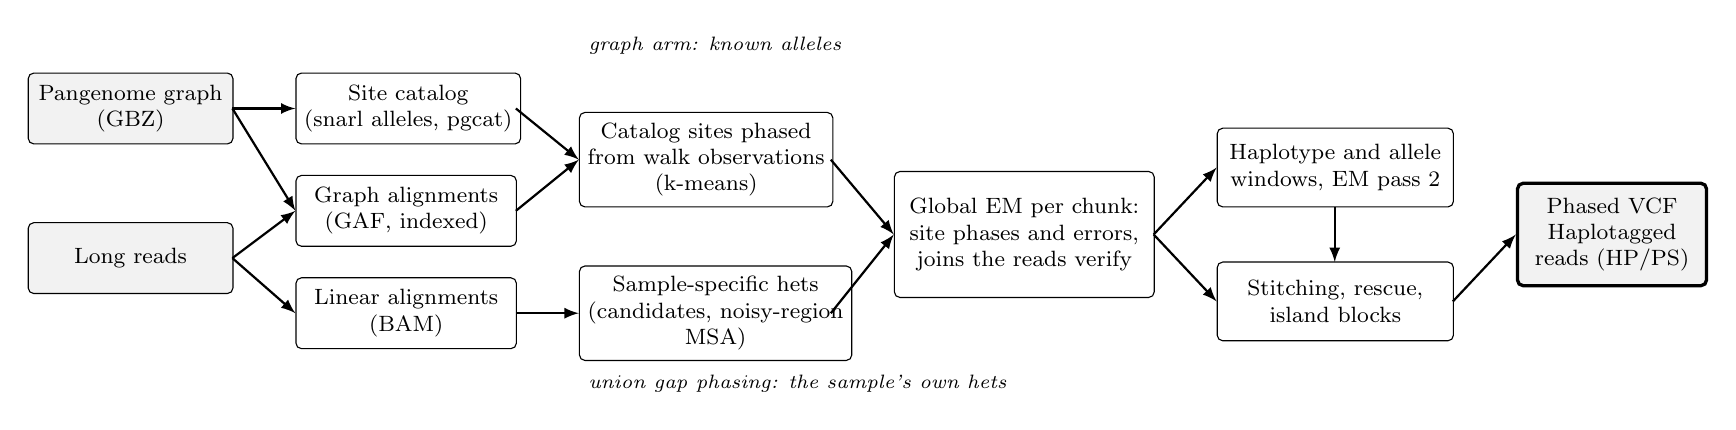
\begin{tikzpicture}
\node[inbox, minimum width=2.6cm, minimum height=0.9cm, anchor=west] (graph) at (0.0,4.2) {Pangenome graph\\(GBZ)};
\node[inbox, minimum width=2.6cm, minimum height=0.9cm, anchor=west] (reads) at (0.0,2.3) {Long reads};
\node[box, minimum width=2.8cm, minimum height=0.9cm, anchor=west] (catalog) at (3.4,4.2) {Site catalog\\(snarl alleles, pgcat)};
\node[box, minimum width=2.8cm, minimum height=0.9cm, anchor=west] (gaf) at (3.4,2.9) {Graph alignments\\(GAF, indexed)};
\node[box, minimum width=2.8cm, minimum height=0.9cm, anchor=west] (bam) at (3.4,1.6) {Linear alignments\\(BAM)};
\node[box, minimum width=3.2cm, minimum height=1.2cm, anchor=west] (clean) at (7.0,3.55) {Catalog sites phased\\from walk observations\\(k-means)};
\node[box, minimum width=3.2cm, minimum height=1.2cm, anchor=west] (solve) at (7.0,1.6) {Sample-specific hets\\(candidates, noisy-region\\MSA)};
\node[box, minimum width=3.3cm, minimum height=1.6cm, anchor=west] (em) at (11.0,2.6) {Global EM per chunk:\\site phases and errors,\\joins the reads verify};
\node[box, minimum width=3.0cm, minimum height=1.0cm, anchor=west] (windows) at (15.1,3.45) {Haplotype and allele\\windows, EM pass 2};
\node[box, minimum width=3.0cm, minimum height=1.0cm, anchor=west] (fill) at (15.1,1.75) {Stitching, rescue,\\island blocks};
\node[outbox, minimum width=2.4cm, minimum height=1.3cm, anchor=west] (out) at (18.9,2.6) {Phased VCF\\Haplotagged\\reads (HP/PS)};
\draw[arr] (2.60,4.20) -- (3.40,4.20);
\draw[arr] (2.60,2.30) -- (3.40,2.90);
\draw[arr] (2.60,2.30) -- (3.40,1.60);
\draw[arr] (2.60,4.20) -- (3.40,2.90);
\draw[arr] (6.20,4.20) -- (7.00,3.55);
\draw[arr] (6.20,2.90) -- (7.00,3.55);
\draw[arr] (6.20,1.60) -- (7.00,1.60);
\draw[arr] (10.20,3.55) -- (11.00,2.60);
\draw[arr] (10.20,1.60) -- (11.00,2.60);
\draw[arr] (14.30,2.60) -- (15.10,3.45);
\draw[arr] (16.60,2.95) -- (16.60,2.25);
\draw[arr] (14.30,2.60) -- (15.10,1.75);
\draw[arr] (18.10,1.75) -- (18.90,2.60);
\node[font=\scriptsize\itshape, anchor=west] at (7.0,5.0) {graph arm: known alleles};
\node[font=\scriptsize\itshape, anchor=west] at (7.0,0.7) {union gap phasing: the sample's own hets};
\end{tikzpicture}}
\caption{pgphase's pipeline. The graph arm phases the sites of a pangenome graph's catalog from the walks the reads' graph alignments take through them; with a linear alignment, union gap phasing adds the sample's own heterozygous variants, and one expectation-maximization phases all sites, joining blocks only where reads verify the join. Reads still unlabelled are phased from local windows, rescue and island blocks.}\label{fig:overview}
\end{figure*}


\subsection{Site catalog and read evidence from a pangenome graph}

The catalog is built once per graph (\texttt{build-snarl-catalog}, from a GBZ graph \citep{Siren2022}): each snarl \citep{Paten2018} of the graph is a site, its reference allele the walk of the reference path through it and its alternative alleles the distinct walks of the haplotype paths, ordered by how many haplotypes take them. The reads' graph alignments are indexed once by reference position (\texttt{index-gaf}). For each chunk, every read crossing a site contributes the allele whose walk its own alignment follows; the identity of an allele is its walk, so two reads carry the same allele exactly when they take the same path through the site. A multi-allelic site is split into one reference-against-alternative contrast per alternative allele, and sites are kept by depth and allele fraction. Indels in homopolymers, tandem repeats and low-complexity sequence are set apart as noisy candidates, which do not take part in the first solve.

\subsection{Phasing the catalog sites}

The catalog's clean heterozygous sites are phased first by k-means clustering of the reads on their alleles, the algorithm of longcallD \citep{Gao2026} applied to walk observations. With a BAM, each graph SNP is checked against the bases of well-mapped reads: one whose reference base no such read shows, and no deletion explains, is reclassified homozygous. Where a read takes a walk that differs from a selected allele only away from a SNP, the walk is read as that SNP's allele, so that reads whose alignment takes a rarer path through a site still vote. The clean solve's labels start the joint solve below.

\subsection{The sample's own heterozygous variants}

With a BAM, each chunk is also solved from its linear alignments, by the alignment pipeline pgphase ports from longcallD \citep{Gao2026}: candidate variants from the reads' differences to the reference, classified by depth, allele fraction and sequence context, with noisy regions up to 2~kb resolved by aligning each haplotype's reads with partial order alignment \citep{Gao2021}. Its clean heterozygous variants, and those verified by the multiple sequence alignment, join the chunk's sites with their per-read alleles. A verified noisy variant must be seen by two reads of mapping quality 30 on each of its two alleles, and no injected site may be read by more than 1.5 times the chunk's median depth: at a collapsed duplication the two "alleles" are the copies, and a run of such sites agrees with itself perfectly. Variants that fail these rules still label reads, but only as islands (Section 2.7). The same indel placed at several copies of a repeat becomes one site; calls inside a catalog site of up to 2~kb only give alleles to reads the graph left without one there; reads only the linear alignment holds are added. At injected indels, every read crossing the site without a call is realigned to the two alleles in reference context and takes the closer one, with a per-read error of \(1/(1+e^{3m})\) for a margin of \(m\) edits. At catalog SNPs a read's graph allele is replaced by its aligned base where the two disagree: measured against the parents, the alignment's base was right in about 90\% of such conflicts.

\subsection{One expectation-maximization over all sites}

Every site with two observed alleles, from the catalog or the sample, gets a phase \(h_s\in\{0,1\}\) and an error rate \(\varepsilon_s\), and every read \(r\) a posterior probability of each haplotype. With \(x_{rs}\) the allele read \(r\) shows at site \(s\) and \(e_{rs}\) the per-read error of that call where one is known, a read on haplotype \(a\) has likelihood

\begin{equation}
L_r(a) = \prod_{s} \bigl(1-\varepsilon_{rs}\bigr)^{[x_{rs} = h_s \oplus a]}\, \varepsilon_{rs}^{[x_{rs} \neq h_s \oplus a]},
\end{equation}

where \(\varepsilon_{rs} = 1-(1-\varepsilon_s)(1-e_{rs})\) combines the site's error with the call's, and expectation-maximization \citep{Dempster1977} alternates the reads' posteriors with the sites' phases and errors. A site's error is the weighted disagreement of its reads, shrunk toward the median error of the sites of its class in the chunk (clean catalog heterozygotes, other catalog sites, injected sites and local windows, each split by whether the site is a one-base length difference) by five pseudo-reads, an empirical Bayes prior that keeps a noisy repeat call from overruling a clean SNP that shares its reads. Only reads of mapping quality 20 or more teach the model; the others are scored against it and labelled. A site whose rarer allele is held by fewer than a quarter of its reads is left out: a skewed split is the signature of a paralog or an error. After the first iterations, the solve tries switch moves, flipping every site past the boundary whose flip most increases the likelihood. A site whose learned error is 0.3 or more is reported unphased and labels no read; a read is labelled in the block where its own evidence is strongest when its posterior there is at least 0.8.

\subsection{Joining blocks only where reads verify the join}

A block ends wherever flipping everything after a boundary would cost less than 4 log-likelihood units, or fewer than two reads carry evidence on both sides: one molecule can be chimeric or misplaced. Beyond that, pgphase restricts which sites can carry a join at all, because a wrong join flips every read past it:

\begin{enumerate}
  \item \textbf{One-base length differences are weak.} A homopolymer length call in a homozygous stretch looks like a heterozygous site; a join that holds only through such sites needs a margin of 10 log units instead of 4.
  \item \textbf{Strong joins need reads.} A join counts as strong only when at least four reads carry evidence at reliable, non-weak sites on both sides of the boundary.
  \item \textbf{Collapsed duplications and poorly mapped sites carry no joins.} A site called by more than twice the chunk's median number of reads, or by more than 1.3 times with its rarer allele under 40\% of them, or whose reads' mean mapping quality is under 40, labels reads but joins nothing.
  \item \textbf{One locus, one vote.} A local window and a call inside it, or several records of one event within 30~bp whose reads split the same way, are counted once.
  \item \textbf{No hinges.} A block that hangs on a single site with weak joins on both sides, crossed by no read, is cut at the weaker join.
\end{enumerate}

These rules leave more, shorter blocks where the reads cannot verify a join, and the reads inside each block phased correctly.

\subsection{Labels for the remaining reads, and output}

Reads the solve leaves unlabelled are labelled from evidence the solve does not vote with. Local haplotype windows (up to 2~kb) contrast the two haplotype sequences of a noisy locus, each built as the medoid of reads labelled on either side; allele windows contrast the two exact alleles of a heterozygous indel the solve does not observe, including two-allele sites with no reference read; and length windows genotype tandem repeat tracts under a stutter model learned from the chunk. A second pass of the solve uses the first two kinds as sites. A read whose calls in a block all agree takes the block's label from posterior 0.7, and a read still unlabelled is phased by its own call at one site that cannot vote, in a block of that site alone, an \emph{island} that never joins anything, so that a wrong island costs only its own reads. Chunks are joined by the reads they share, only when one orientation leads by at least three reads and 90\%; a read without a label takes one from the phase set its alleles at excluded sites associate with (one-sided binomial test, \(p \le 0.01\)). In the VCF, a phase set whose heterozygotes all lie at one locus is written unphased, as are SNPs of learned error 0.1 or more and indels of 0.25 or more.

\subsection{Evaluation}

\textbf{Data.} HG002 \citep{Zook2016} PacBio HiFi reads (DRAFT: source and chemistry) were aligned with vg Giraffe v1.73.0 \citep{Siren2021} (HiFi preset, minimizers \(k=31\), \(w=50\)) to a 16-haplotype sample \citep{Siren2024} of the Human Pangenome Reference Consortium release 2 Minigraph-Cactus graph on CHM13 \citep{Liao2023,Hickey2024,HPRC2}, from which HG002 and its parents had been removed (229 assembled samples, CHM13 and GRCh38), and surjected onto CHM13 \citep{Nurk2022}; they covered chr19 at 59-fold. The catalog was built from the whole graph. Every tool was given the same reads: pgphase their graph alignments and the surjected BAM, the other tools the BAM. HiPhase 1.6.0, LongPhase 2.0.2 and WhatsHap 2.8, by default and with \texttt{-{}-distrust-genotypes} (WhatsHap-dg), phased DeepVariant 1.10.0 calls (PACBIO model) made on the same BAM; longcallD (v0.0.11) called and phased its own. pgphase was developed on chr12, chr17, chr18, chr19 and chr20, whose truth guided its rules and constants; chr6, chr16 and chr21, and the MHC of chr6, were held out until the comparison.

\textbf{Truth.} Each read's parent of origin was found by aligning it with minimap2 \citep{Li2018} to both haplotypes of the HG002 v1.1 assembly \citep{Hansen2025} and taking the better alignment with HipHap \citep{HipHap}, which also scores the confidence of the assignment (HapQ). Truth heterozygous variants are the Q100 HG002 small-variant benchmark on CHM13 \citep{Hansen2025}.

\textbf{Read metrics.} A primary read is \emph{phaseable} when its alignment spans a heterozygous truth variant. Each phase set takes the parental orientation of the majority of its truth-labelled reads; a read is \emph{correct} when its tag agrees with it, \emph{discordant} when it does not, and \emph{unphased} when it has no tag. Reads are on the \emph{arms} or in the centromeric and pericentromeric satellites of CHM13's cenSat annotation \citep{Altemose2022} (for chr21, its acrocentric short arm too). We also report the discordant reads whose parental label is confident (HapQ $\ge$ 30): below HapQ 10, every tool is 25--37\% discordant, and most such reads carry the other parent's bases at their own clean SNVs, so their label rather than their phase is wrong.

\textbf{Variant metrics.} A tool's phased heterozygous biallelic records are matched to the truth by position, reference and alternative allele. Within a phase set, a single matched heterozygote whose orientation disagrees with its agreeing neighbours is a \emph{flip} and a lasting change a \emph{switch}. In repeats, the same haplotypes can be written as different records, and a record-level scorer then counts switches that are not. We therefore class each switch by sequence: around each of the two heterozygotes bounding it, a window of 75~bp on either side, grown until no record of either VCF crosses its edges (at most 20~kb), the tool's two haplotype sequences are compared with the truth's by edit distance, and each window pairs them in the cheaper way. A switch is \emph{real} when the two windows pair them in opposite ways, \emph{representation} when both pair them the same way, and \emph{undecided} when either window's two pairings are within 30\% (or 2 edits) of each other.

% Generated by tools/paper/render.py from main_text.py; edit the source there, not this file.
\section{Results}

\subsection{More reads phased correctly, fewer misphased}

Over the eight chromosomes, 2{,}623,162 reads on the arms span a heterozygous truth variant. pgphase phased 99.08\% of them correctly, 0.67\% discordantly and left 0.25\% unphased (Table~\ref{tab:reads}). The best of the other tools, HiPhase, phased 94.41\% correctly: pgphase phased 122{,}476 more reads correctly, and left 6.1 times fewer reads discordant or unphased than the tool with the fewest such reads, HiPhase. It phased the most reads correctly on every chromosome, and on 6 of the eight left the fewest discordant reads; on chr20 and chr21, LongPhase left fewer, while leaving many more reads unphased (Fig.~\ref{fig:accuracy}). Among reads whose parental label is confident, pgphase phased 4{,}369 discordantly, against 17{,}918 for longcallD, the lowest of the others.

% Generated by tools/paper/render.py from main_text.py; edit the source there, not this file.
\begin{table*}[t]
\caption{Phaseable reads on the chromosome arms that each tool phases correctly. A read is phaseable when its alignment spans a heterozygous truth variant; it is correct when its haplotype tag agrees with the parental orientation its phase set takes over its truth-labelled reads, discordant when it does not, unphased when it has none. Per chromosome the share of phaseable reads phased correctly (\%); below, the totals over the eight chromosomes, and the discordant reads whose parental label is confident (HapQ $\ge$ 30). The MHC lies inside chr6 and is not added to the totals. Best in bold. WhatsHap-dg: WhatsHap with \texttt{-{}-distrust-genotypes}.}\label{tab:reads}
\centering\footnotesize
\setlength{\tabcolsep}{4pt}
\begin{tabular}{@{}lrrrrrr@{}}
\toprule
Chromosome & pgphase & HiPhase & LongPhase & WhatsHap & WhatsHap-dg & longcallD \\
\midrule
\multicolumn{7}{@{}l}{\emph{Used in development}} \\
chr12 & \textbf{99.48} & 95.70 & 93.77 & 92.51 & 94.47 & 92.30 \\
chr17 & \textbf{98.66} & 93.93 & 90.67 & 87.92 & 89.03 & 87.26 \\
chr18 & \textbf{99.42} & 94.72 & 92.21 & 91.01 & 91.50 & 91.68 \\
chr19 & \textbf{98.40} & 92.54 & 90.50 & 85.54 & 89.66 & 89.78 \\
chr20 & \textbf{99.23} & 95.39 & 92.95 & 90.90 & 93.10 & 91.34 \\
\multicolumn{7}{@{}l}{\emph{Held out}} \\
chr6 & \textbf{99.24} & 94.54 & 91.68 & 91.67 & 92.27 & 90.92 \\
chr16 & \textbf{98.39} & 91.29 & 91.62 & 85.85 & 88.48 & 85.78 \\
chr21 & \textbf{99.15} & 97.02 & 92.66 & 93.55 & 94.03 & 91.35 \\
\multicolumn{7}{@{}l}{\emph{Region of chr6, held out}} \\
MHC (chr6:28.5--34.0~Mb) & \textbf{99.31} & 96.95 & 93.81 & 94.92 & 95.23 & 90.63 \\
\multicolumn{7}{@{}l}{\emph{All eight chromosomes}} \\
Correct (\%) & \textbf{99.08} & 94.41 & 92.11 & 90.28 & 91.81 & 90.28 \\
Discordant & \textbf{17{,}676} & 81{,}049 & 29{,}439 & 125{,}340 & 83{,}852 & 31{,}773 \\
Unphased & \textbf{6{,}432} & 65{,}535 & 177{,}500 & 129{,}614 & 130{,}987 & 223{,}210 \\
Discordant, HapQ $\ge$ 30 & \textbf{4{,}369} & 64{,}722 & 21{,}505 & 105{,}538 & 69{,}813 & 17{,}918 \\
\bottomrule
\end{tabular}
\end{table*}


% Generated by tools/paper/render.py from main_text.py; edit the source there, not this file.
\begin{figure*}[t]
\centering
\resizebox{\textwidth}{!}{\begin{tikzpicture}
\node[font=\bfseries] at (-2.3,3.95) {a};
\draw[gray!25] (0.00,-0.35) -- (0.00,3.40);\node[below,font=\scriptsize] at (0.00,-0.35) {0};
\draw[gray!25] (1.24,-0.35) -- (1.24,3.40);\node[below,font=\scriptsize] at (1.24,-0.35) {2};
\draw[gray!25] (2.48,-0.35) -- (2.48,3.40);\node[below,font=\scriptsize] at (2.48,-0.35) {4};
\draw[gray!25] (3.72,-0.35) -- (3.72,3.40);\node[below,font=\scriptsize] at (3.72,-0.35) {6};
\draw[gray!25] (4.96,-0.35) -- (4.96,3.40);\node[below,font=\scriptsize] at (4.96,-0.35) {8};
\draw[gray!25] (6.20,-0.35) -- (6.20,3.40);\node[below,font=\scriptsize] at (6.20,-0.35) {10};
\node[font=\small] at (3.10,-1.05) {\% of phaseable arm reads};
\fill[cpgphase] (0,2.900) rectangle (0.418,3.300);
\fill[cpgphase!35] (0.418,2.900) rectangle (0.570,3.300);
\node[left,font=\small\bfseries] at (-0.05,3.100) {pgphase};
\node[right,font=\scriptsize\bfseries] at (0.620,3.100) {0.92\%};
\fill[chiphase] (0,2.280) rectangle (1.916,2.680);
\fill[chiphase!35] (1.916,2.280) rectangle (3.465,2.680);
\node[left,font=\small] at (-0.05,2.480) {HiPhase};
\node[right,font=\scriptsize] at (3.515,2.480) {5.59\%};
\fill[clongphase] (0,1.660) rectangle (0.696,2.060);
\fill[clongphase!35] (0.696,1.660) rectangle (4.891,2.060);
\node[left,font=\small] at (-0.05,1.860) {LongPhase};
\node[right,font=\scriptsize] at (4.941,1.860) {7.89\%};
\fill[cwhatshapopt] (0,1.040) rectangle (1.982,1.440);
\fill[cwhatshapopt!35] (1.982,1.040) rectangle (5.078,1.440);
\node[left,font=\small] at (-0.05,1.240) {WhatsHap-dg};
\node[right,font=\scriptsize] at (5.128,1.240) {8.19\%};
\fill[cwhatshap] (0,0.420) rectangle (2.962,0.820);
\fill[cwhatshap!35] (2.962,0.420) rectangle (6.026,0.820);
\node[left,font=\small] at (-0.05,0.620) {WhatsHap};
\node[right,font=\scriptsize] at (6.076,0.620) {9.72\%};
\fill[clongcalld] (0,-0.200) rectangle (0.751,0.200);
\fill[clongcalld!35] (0.751,-0.200) rectangle (6.027,0.200);
\node[left,font=\small] at (-0.05,0.000) {longcallD};
\node[right,font=\scriptsize] at (6.077,0.000) {9.72\%};
\fill[black!75] (2.3,3.55) rectangle (2.6,3.75);\node[right,font=\scriptsize] at (2.6,3.65) {misphased};
\fill[black!25] (4.2,3.55) rectangle (4.5,3.75);\node[right,font=\scriptsize] at (4.5,3.65) {unphased};
\node[font=\bfseries] at (8.30,3.95) {b};
\draw[gray!25] (10.427,-0.35) -- (10.427,4.37);\node[below,font=\scriptsize] at (10.427,-0.35) {0.5};
\draw[gray!25] (11.549,-0.35) -- (11.549,4.37);\node[below,font=\scriptsize] at (11.549,-0.35) {1};
\draw[gray!25] (12.672,-0.35) -- (12.672,4.37);\node[below,font=\scriptsize] at (12.672,-0.35) {2};
\draw[gray!25] (14.155,-0.35) -- (14.155,4.37);\node[below,font=\scriptsize] at (14.155,-0.35) {5};
\draw[gray!25] (15.278,-0.35) -- (15.278,4.37);\node[below,font=\scriptsize] at (15.278,-0.35) {10};
\draw[gray!25] (16.400,-0.35) -- (16.400,4.37);\node[below,font=\scriptsize] at (16.400,-0.35) {20};
\node[font=\small] at (13.00,-1.05) {misphased or unphased (\%, log scale)};
\draw[gray!15, line width=3pt] (9.60,4.067) -- (16.40,4.067);\node[left,font=\small] at (9.55,4.067) {chr12};
\draw[gray!15, line width=3pt] (9.60,3.559) -- (16.40,3.559);\node[left,font=\small] at (9.55,3.559) {chr17};
\draw[gray!15, line width=3pt] (9.60,3.050) -- (16.40,3.050);\node[left,font=\small] at (9.55,3.050) {chr18};
\draw[gray!15, line width=3pt] (9.60,2.542) -- (16.40,2.542);\node[left,font=\small] at (9.55,2.542) {chr19};
\draw[gray!15, line width=3pt] (9.60,2.034) -- (16.40,2.034);\node[left,font=\small] at (9.55,2.034) {chr20};
\draw[gray!15, line width=3pt] (9.60,1.017) -- (16.40,1.017);\node[left,font=\small] at (9.55,1.017) {chr6};
\draw[gray!15, line width=3pt] (9.60,0.508) -- (16.40,0.508);\node[left,font=\small] at (9.55,0.508) {chr16};
\draw[gray!15, line width=3pt] (9.60,0.000) -- (16.40,0.000);\node[left,font=\small] at (9.55,0.000) {chr21};
\node[rotate=-90,font=\scriptsize\itshape,black!65] at (16.75,3.050) {development};
\node[rotate=-90,font=\scriptsize\itshape,black!65] at (16.75,0.508) {not tuned};
\fill[chiphase, draw=white, line width=0.3pt] (13.910,4.067) circle (0.075);
\fill[chiphase, draw=white, line width=0.3pt] (14.469,3.559) circle (0.075);
\fill[chiphase, draw=white, line width=0.3pt] (14.242,3.050) circle (0.075);
\fill[chiphase, draw=white, line width=0.3pt] (14.803,2.542) circle (0.075);
\fill[chiphase, draw=white, line width=0.3pt] (14.023,2.034) circle (0.075);
\fill[chiphase, draw=white, line width=0.3pt] (14.298,1.017) circle (0.075);
\fill[chiphase, draw=white, line width=0.3pt] (15.053,0.508) circle (0.075);
\fill[chiphase, draw=white, line width=0.3pt] (13.316,0.000) circle (0.075);
\fill[clongphase, draw=white, line width=0.3pt] (14.510,4.067) circle (0.075);
\fill[clongphase, draw=white, line width=0.3pt] (15.165,3.559) circle (0.075);
\fill[clongphase, draw=white, line width=0.3pt] (14.874,3.050) circle (0.075);
\fill[clongphase, draw=white, line width=0.3pt] (15.194,2.542) circle (0.075);
\fill[clongphase, draw=white, line width=0.3pt] (14.712,2.034) circle (0.075);
\fill[clongphase, draw=white, line width=0.3pt] (14.979,1.017) circle (0.075);
\fill[clongphase, draw=white, line width=0.3pt] (14.991,0.508) circle (0.075);
\fill[clongphase, draw=white, line width=0.3pt] (14.777,0.000) circle (0.075);
\fill[cwhatshap, draw=white, line width=0.3pt] (14.810,4.067) circle (0.075);
\fill[cwhatshap, draw=white, line width=0.3pt] (15.584,3.559) circle (0.075);
\fill[cwhatshap, draw=white, line width=0.3pt] (15.105,3.050) circle (0.075);
\fill[cwhatshap, draw=white, line width=0.3pt] (15.874,2.542) circle (0.075);
\fill[cwhatshap, draw=white, line width=0.3pt] (15.125,2.034) circle (0.075);
\fill[cwhatshap, draw=white, line width=0.3pt] (14.981,1.017) circle (0.075);
\fill[cwhatshap, draw=white, line width=0.3pt] (15.840,0.508) circle (0.075);
\fill[cwhatshap, draw=white, line width=0.3pt] (14.567,0.000) circle (0.075);
\fill[cwhatshapopt, draw=white, line width=0.3pt] (14.317,4.067) circle (0.075);
\fill[cwhatshapopt, draw=white, line width=0.3pt] (15.428,3.559) circle (0.075);
\fill[cwhatshapopt, draw=white, line width=0.3pt] (15.014,3.050) circle (0.075);
\fill[cwhatshapopt, draw=white, line width=0.3pt] (15.332,2.542) circle (0.075);
\fill[cwhatshapopt, draw=white, line width=0.3pt] (14.677,2.034) circle (0.075);
\fill[cwhatshapopt, draw=white, line width=0.3pt] (14.860,1.017) circle (0.075);
\fill[cwhatshapopt, draw=white, line width=0.3pt] (15.507,0.508) circle (0.075);
\fill[cwhatshapopt, draw=white, line width=0.3pt] (14.441,0.000) circle (0.075);
\fill[clongcalld, draw=white, line width=0.3pt] (14.854,4.067) circle (0.075);
\fill[clongcalld, draw=white, line width=0.3pt] (15.670,3.559) circle (0.075);
\fill[clongcalld, draw=white, line width=0.3pt] (14.980,3.050) circle (0.075);
\fill[clongcalld, draw=white, line width=0.3pt] (15.313,2.542) circle (0.075);
\fill[clongcalld, draw=white, line width=0.3pt] (15.045,2.034) circle (0.075);
\fill[clongcalld, draw=white, line width=0.3pt] (15.121,1.017) circle (0.075);
\fill[clongcalld, draw=white, line width=0.3pt] (15.848,0.508) circle (0.075);
\fill[clongcalld, draw=white, line width=0.3pt] (15.043,0.000) circle (0.075);
\fill[cpgphase, draw=white, line width=0.3pt] (10.498,4.067) circle (0.11);
\fill[cpgphase, draw=white, line width=0.3pt] (12.028,3.559) circle (0.11);
\fill[cpgphase, draw=white, line width=0.3pt] (10.658,3.050) circle (0.11);
\fill[cpgphase, draw=white, line width=0.3pt] (12.314,2.542) circle (0.11);
\fill[cpgphase, draw=white, line width=0.3pt] (11.131,2.034) circle (0.11);
\fill[cpgphase, draw=white, line width=0.3pt] (11.114,1.017) circle (0.11);
\fill[cpgphase, draw=white, line width=0.3pt] (12.323,0.508) circle (0.11);
\fill[cpgphase, draw=white, line width=0.3pt] (11.277,0.000) circle (0.11);
\end{tikzpicture}}
\caption{Phaseable reads on the chromosome arms that each tool misphases or leaves unphased. (a) Over the eight chromosomes, the share misphased (discordant, dark) and unphased (light), tools ordered by their total. (b) Per chromosome, the share misphased or unphased (log scale); chr6, chr16 and chr21 were not used for tuning; colours as in (a). Lower is better.}\label{fig:accuracy}
\end{figure*}


The margin held on chromosomes the method was not developed on. On the held-out chr6, chr16 and chr21, pgphase phased 2.1 to 6.8 percentage points more phaseable reads correctly than the best other tool on each, against 3.8 to 5.9 points on the development chromosomes. In the MHC, whose HLA genes are among the most polymorphic of the genome, it phased 99.31\% correctly, against 96.95\% for HiPhase.

\subsection{Switch errors}

pgphase made 58 switch errors on the arms of the eight chromosomes, against 105 for LongPhase, the fewest among the others, and 178 for HiPhase (Table~\ref{tab:switches}). Classed by haplotype sequence, 10 of pgphase's switches were real, 13 wrote the truth's haplotypes with different records, and 35 were undecided, against 41 to 220 real switches for the other tools. Undecided switches are mostly tandem repeats where neither of a tool's haplotypes matches either of the truth's, so that no pairing is better than the other. pgphase made 81 flips, against 80 for LongPhase.

% Generated by tools/paper/render.py from main_text.py; edit the source there, not this file.
\begin{table*}[t]
\caption{Switch and flip errors on the chromosome arms and switch errors in the centromeric and pericentromeric satellites, phased truth heterozygotes and blocks, over the eight chromosomes. A switch is a lasting change of a phase set's orientation against the truth between consecutive truth-matched heterozygotes, a flip a single heterozygote out of line with its neighbours. Each switch is classified by comparing the tool's two haplotype sequences around its two heterozygotes with the truth's (Section 2.8): \emph{real}, a genuine phasing error, when the two windows pair the tool's haplotypes with the truth's in opposite ways; \emph{representation} when both pair them the same way (the tool writes the same haplotypes as the truth with different records); \emph{undecided} when either window's two pairings are within 30\% of each other (or 2 edits). Per 10k: arm switches per 10{,}000 phased truth heterozygotes on the arms. Phased hets: truth-matched heterozygous variants written phased. Phase sets summed over the chromosomes, block N50 the median of the per-chromosome N50s.}\label{tab:switches}
\centering\footnotesize
\setlength{\tabcolsep}{4pt}
\begin{tabular}{@{}lrrrrrrrrrr@{}}
\toprule
 & \multicolumn{5}{c}{Arm switches} & \multicolumn{1}{c}{Satellites} & \multicolumn{2}{c}{Variants} & \multicolumn{2}{c}{Blocks} \\ \cmidrule(lr){2-6}\cmidrule(lr){7-7}\cmidrule(lr){8-9}\cmidrule(lr){10-11}
Tool & All & Per 10k & Real & Repr. & Undec. & Switches & Arm flips & Phased hets & Phase sets & N50 (kb) \\
\midrule
pgphase & \textbf{58} & \textbf{0.83} & \textbf{10} & 13 & 35 & \textbf{42} & 81 & 716{,}046 & 4{,}431 & 587 \\
HiPhase & 178 & 2.68 & 119 & 2 & 57 & 402 & 105 & 684{,}672 & \textbf{2{,}216} & \textbf{832} \\
LongPhase & 105 & 1.83 & 41 & 5 & 59 & 349 & \textbf{80} & 593{,}681 & 2{,}720 & 610 \\
WhatsHap & 364 & 5.47 & 220 & 32 & 112 & 471 & 997 & 685{,}315 & 2{,}378 & 763 \\
WhatsHap-dg & 208 & 3.15 & 130 & 10 & 68 & 363 & 228 & 679{,}677 & 2{,}511 & 740 \\
longcallD & 200 & 2.83 & 115 & 36 & 49 & 177 & 172 & \textbf{726{,}046} & 4{,}589 & 414 \\
\bottomrule
\end{tabular}
\end{table*}


\subsection{Phased variants and blocks}

pgphase phased 716{,}046 truth heterozygous variants, against 726{,}046 for longcallD, the most of the others (Table~\ref{tab:switches}). Its blocks are shorter than HiPhase's: 4{,}431 phase sets against 2{,}216, a median block N50 of 587~kb against 832~kb. The difference is where the join rules refuse to join: across collapsed duplications and stretches read only at low mapping quality, where each site is its own block. The reads there are phased within their blocks, and a join that the reads cannot verify is exactly what flips them.

\subsection{Centromeres}

In centromeric and pericentromeric satellites, where reads map ambiguously and copies differ by few bases, pgphase phased 93{,}251 reads correctly at 5.4 correct reads per discordant one (Table~\ref{tab:cen}). LongPhase phased 86{,}567 correctly at 2.6 per discordant read, phasing more of them but with more of them wrong. longcallD reached 18.0 correct reads per discordant one by phasing few: 42{,}138 correctly, with 104{,}573 left unphased.

% Generated by tools/paper/render.py from main_text.py; edit the source there, not this file.
\begin{table}[t]
\caption{Phaseable reads in centromeric and pericentromeric satellites (one interval per chromosome, Supplementary Table S4) over the eight chromosomes, and the ratio of correct to discordant reads.}\label{tab:cen}
\centering\footnotesize
\setlength{\tabcolsep}{4pt}
\begin{tabular}{@{}lrrrr@{}}
\toprule
Tool & Correct & Discordant & Unphased & Correct : discordant \\
\midrule
pgphase & \textbf{93{,}251} & 17{,}427 & 38{,}375 & 5.4 \\
HiPhase & 62{,}162 & 13{,}370 & 73{,}521 & 4.6 \\
LongPhase & 86{,}567 & 33{,}538 & \textbf{28{,}948} & 2.6 \\
WhatsHap & 46{,}997 & 4{,}107 & 97{,}949 & 11.4 \\
WhatsHap-dg & 47{,}073 & 3{,}906 & 98{,}074 & 12.1 \\
longcallD & 42{,}138 & \textbf{2{,}342} & 104{,}573 & \textbf{18.0} \\
\bottomrule
\end{tabular}
\end{table}


\subsection{Running time and memory}

On the 5 chromosomes where every tool ran with the same threads, pgphase took 7.1 minutes with six, against 18.4 for HiPhase and 3.3 for LongPhase; on chr6, 147~s against 459~s and 92~s (Table~\ref{tab:resources}). Its time includes finding the sample's variants and writing the haplotagged reads, while the others' excludes DeepVariant. It needed up to 8.5~GB of memory, more than the phasers given DeepVariant's calls.

% Generated by tools/paper/render.py from main_text.py; edit the source there, not this file.
\begin{table}[t]
\caption{Wall-clock time and peak memory (GNU time) on one machine with 10 cores, on the five chromosomes where every multi-threaded tool ran with 6 threads (chr17, chr19, chr6, chr16, chr21): chr6, the largest, then the total time and the largest peak memory. The DeepVariant-based phasers' times exclude DeepVariant; pgphase's include its own variant discovery and the haplotagged reads, and exclude graph alignment.}\label{tab:resources}
\centering\footnotesize
\setlength{\tabcolsep}{4pt}
\begin{tabular}{@{}lrrrr@{}}
\toprule
Tool & Threads & chr6 (s) & Total (min) & Memory (GB) \\
\midrule
pgphase & 6 & 147 & 7.1 & 8.5 \\
HiPhase & 6 & 459 & 18.4 & 0.5 \\
LongPhase & 6 & 92 & 3.3 & 3.4 \\
WhatsHap & 1 & 1004 & 41.9 & 1.7 \\
WhatsHap-dg & 1 & 1113 & 46.8 & 2.1 \\
longcallD & 6 & 235 & 8.0 & 13.3 \\
\bottomrule
\end{tabular}
\end{table}


% Generated by tools/paper/render.py from main_text.py; edit the source there, not this file.
\section{Discussion}

Phasers are usually compared through their phased variants, but many uses of long-read phasing depend on the reads: a read left unphased is lost to every haplotype-resolved analysis, and a block joined in the wrong orientation misassigns all of its reads. On these terms pgphase phased more reads correctly than the tools we compared it with, on every chromosome we tested. Two of its design choices are the likely reasons, although we have not measured their contributions separately. First, it has more sites to phase reads with: the graph's known alleles, observed in the reads' graph alignments rather than called, and the sample's own heterozygous variants. Second, it is conservative in joining blocks: sites at collapsed duplications, poorly mapped sites and homopolymer length calls still label the reads that cross them but cannot join two blocks. The cost of the second is more and shorter blocks than HiPhase produces where the reads cannot verify how blocks connect.

Our evaluation has limits. All tools were given reads aligned to a pangenome graph and surjected onto CHM13, not the linear alignments (for example from minimap2 or pbmm2) the other tools are usually run on, and their accuracy with such alignments may differ. We evaluated one sample and one sequencing technology on eight chromosomes; other samples, ONT reads and other graphs remain to be tested. The development chromosomes shaped pgphase's rules and thresholds, and although the chromosomes not used for tuning showed a similar margin, they were scored during development. The read truth relies on alignment to the parental assemblies, and its labels are least reliable where the parental haplotypes are most similar.

pgphase also has limits of its own. Its catalog holds only the alleles of the genomes in the graph: at a tandem repeat whose expansion in the sample no genome shares, a read's graph alignment follows the closest known walk, and most of the switches we could not classify are of this kind. Representing such alleles from the reads themselves is a natural next step. pgphase also needs graph alignments of the reads and more memory than the phasers it was compared with. Finally, a record-level comparison counts differences of representation in repeats as switch errors; classifying switches by haplotype sequence, as here, or comparing haplotypes rather than records, would make phasers easier to compare.

% Generated by tools/paper/render.py from main_text.py; edit the source there, not this file.
\section*{Author contributions}
Konstantinos Kyriakidis (Conceptualization [lead], Methodology [lead], Software [lead], Validation [lead], Formal analysis [lead], Investigation [lead], Data curation [lead], Visualization [lead], Writing---original draft [lead]), Benedict Paten (Supervision [lead], Writing---review \& editing [equal]).

\section*{Supplementary data}
Supplementary data are available at \emph{Bioinformatics} online.

\section*{Conflict of interest}
None declared.

\section*{Funding}
This work received no specific funding.

\section*{Data availability}
pgphase is available at \url{https://github.com/kokyriakidis/pgphase}; the results reported here are of pgphase 89573ef. The scores behind every table and figure are in the same repository (\texttt{tools/paper/results.json}), from which \texttt{tools/paper/} regenerates this paper. The evaluation scripts, which run every tool and score its output, are available at \url{https://github.com/kokyriakidis/pgphase-dev}, and the exact command of every tool is given in Supplementary Section S7. The HG002 reads (DRAFT: source), the HPRC release 2 graph \citep{HPRC2}, the HG002 v1.1 assembly and the Q100 benchmark \citep{Hansen2025} are publicly available.

\bibliographystyle{oup-abbrvnat}
\bibliography{references}
\end{document}
